\documentclass[tikz,border=5pt]{standalone}
\usepackage{tikz}
\usepackage{tikz-3dplot}
\usepackage{amssymb}
\usepackage{amsmath}
\usepackage{bm}
\usetikzlibrary{arrows.meta}
\usetikzlibrary{arrows}
\usepackage{pstricks}
\usetikzlibrary{patterns}
\usetikzlibrary{fadings}
\usetikzlibrary{shapes.geometric}

\begin{document}

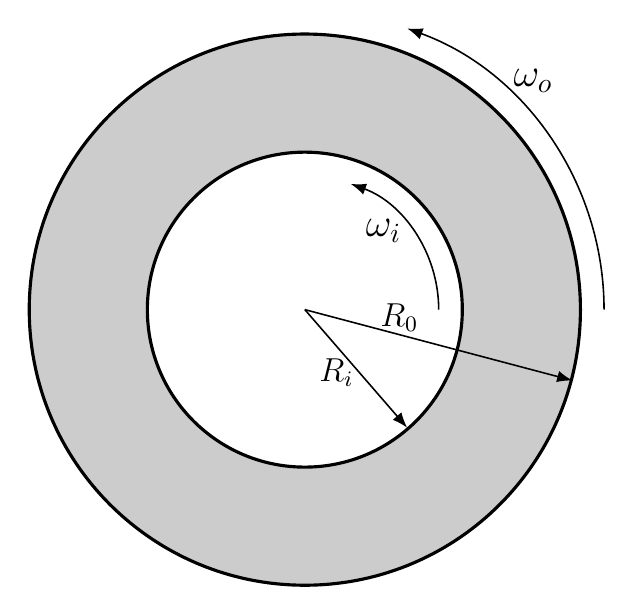
\begin{tikzpicture}

	\tikzset{mybluearrow/.style={-Latex, blue, line width=0.6mm, shorten <=-2pt}}
	\tikzset{myblackarrow/.style={-Latex, black, line width=0.3mm, shorten <=-2pt}}
	\tikzset{myblackarrow/.style={-Latex, black, line width=0.2mm, shorten <=0pt}}

	% Parameters
	\def\Rout{3.5}   % outer radius
	\def\Rin{2}    % inner radius

	%bottom inner circle part

	\fill[gray!40, even odd rule]
	(0,0) circle (\Rout)
	(0,0) circle (\Rin);

	\draw[thick, line width=0.4mm] (0,0) circle (\Rin);

	\draw[thick, line width=0.4mm] (0,0) circle (\Rout);
	\\
	\draw[myblackarrow] (0,0) -- (3.4,-0.9);
	\draw[myblackarrow] (0,0) -- (1.3,-1.5);

	\draw[
		thick,
		myblackarrow
	]
	(\Rin - 0.3,0)
	arc[start angle=0, end angle=70, radius=\Rin-0.3];

	\draw[
		thick,
		myblackarrow
	]
	(\Rout + 0.3,0)
	arc[start angle=0, end angle=70, radius=\Rout+0.3];

	\draw (\Rin-1,\Rin-1)node[]{\Large{${\omega_i}$}};
	\draw (\Rout-0.6,\Rout-0.6)node[]{\Large{${\omega_o}$}};

	\draw (0.4,-0.8)node[]{\large{${R_i}$}};
	\draw (1.2,-0.1)node[]{\large{${R_0}$}};

\end{tikzpicture}

\end{document}
